\section{Yolo You Only Look Once}

\begin{figure}
  \centering
  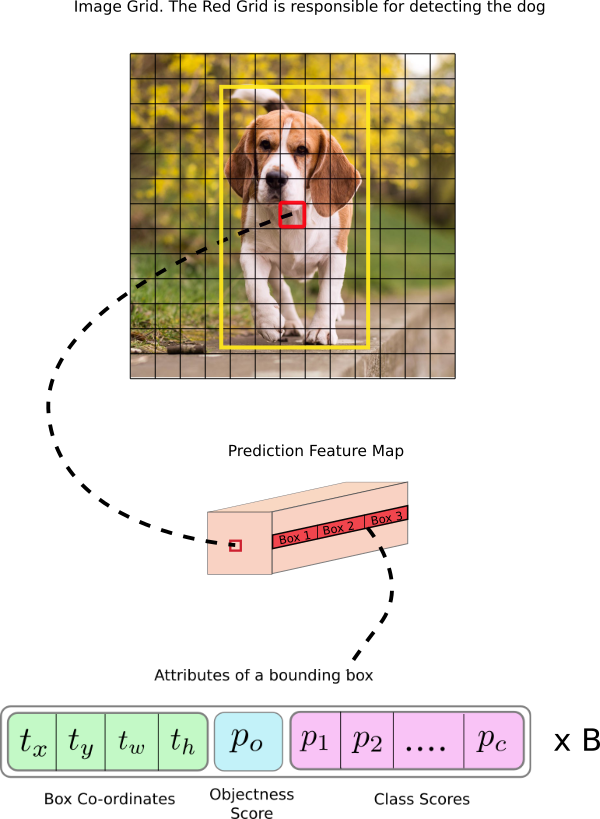
\includegraphics[width=0.8\textwidth]{images/yolo/grid.png}
  \caption{Image Grid}
\end{figure}

\subsection{YoloV1}
\begin{itemize}
  \item Grid Division: YoloV1 divides the input image into an SxS grid. For each grid cell, the model predicts B bounding boxes and confidence scores for those boxes. These scores reflect how confident the model is that the box contains an object and also how accurate it thinks the box is that it predicts.
  \item Bounding Box Prediction: Each bounding box consists of 5 predictions - x, y, w, h, and confidence. The (x, y) coordinates represent the center of the box relative to the bounds of the grid cell. The width and height (w and h) are predicted relative to the whole image. Finally, confidence prediction represents the Intersection over Union (IoU) between the predicted box and any ground truth box.
  \item Class Probability Prediction: Each grid cell also predicts a conditional class probability for C classes. These probabilities are conditioned on the grid cell containing an object.
  \item Output: The output of the network is a tensor of shape SxSx(B*5+C). For each grid cell, this tensor contains the attributes (x, y, w, h, confidence) for B boxes and C class probabilities.
  \item Loss Function: The loss function in YoloV1 is a combination of:
        \begin{itemize}
          \item Localization error (bounding box coordinate error): Measures the errors in the predicted bounding box locations and sizes.
          \item Confidence error: Measures the difference between the predicted confidence scores (how sure the model is that the box contains an object and how well the box fits the object) and the ground truth.
          \item Classification error: Measures the errors in the predicted class probabilities.
        \end{itemize}
\end{itemize}

\subsection{YoloV2}
\begin{itemize}
  \item Multi-Scale Training: YoloV2 introduces the concept of multi-scale training, where the network is trained to predict objects at different scales. This allows the model to detect smaller objects that might have been missed by YoloV1.
  \item Use of Anchor Boxes: YoloV2 introduces the concept of anchor boxes. Instead of directly predicting the coordinates of the bounding boxes, YoloV2 predicts the offsets of predefined anchor boxes. These anchor boxes have different scales and aspect ratios to handle objects of various sizes and shapes. By predicting the offsets, YoloV2 simplifies the task of object detection.
  \item Darknet-19: YoloV2 uses a new network architecture called Darknet-19 for feature extraction. Darknet-19 is a 19-layer network that uses 3x3 filters for feature extraction and 1x1 filters for reducing the dimensionality.
  \item Batch Normalization: YoloV2 uses batch normalization in all of the convolutional layers of Darknet-19. Batch normalization helps to stabilize the learning process and reduces the number of training epochs required.
  \item High Resolution Classifier: YoloV2 starts the training process with a classifier network that is trained on a higher resolution than YoloV1. This helps the network to recognize small objects.
  \item Direct location prediction: YoloV2 predicts the x and y coordinates of the bounding box directly using a sigmoid function, which keeps the prediction between 0 and 1. This helps to constrain the location prediction.
  \item Multi-label Classification: YoloV2 is capable of predicting multiple labels for an object, which is a significant improvement over YoloV1 that could only predict a single label for each object.
\end{itemize}

\subsection{YoloV3}
\begin{itemize}
  \item Three Scales: YoloV3 makes detections at three different scales by using three different sizes of anchor boxes. This is achieved by extracting feature maps from three different layers in the network, allowing the detection of objects of various sizes.
  \item Darknet-53: YoloV3 uses a new network architecture called Darknet-53, which is a hybrid of Darknet-19 (used in YoloV2) and ResNet. Darknet-53 has 53 convolutional layers and is more powerful and efficient than Darknet-19.
  \item Class Prediction: Unlike YoloV2, which uses Softmax for class prediction, YoloV3 uses independent logistic classifiers to calculate the likeliness of input belonging to a specific label. This change was made because Softmax assumes that classes are mutually exclusive, which is not the case in multi-label classification scenarios.
  \item Bounding Box Prediction: YoloV3 predicts an objectness score for each bounding box using logistic regression. This score directly predicts the probability of an object's presence in the bounding box.
  \item Intersection Over Union (IoU) Thresholds: YoloV3 uses multiple Intersection Over Union (IoU) thresholds to evaluate the quality of the bounding boxes. It helps in reducing the duplicate detections of the same object.
\end{itemize}

\subsection{YoloV4}
\begin{itemize}
  \item CSPDarknet53: YoloV4 uses CSPDarknet53 as its backbone network for feature extraction. CSPDarknet53 is a variant of Darknet53 that uses Cross Stage Partial connections (CSP), which can increase the learning capability of the network while reducing computational cost.
  \item Mish Activation Function: YoloV4 uses the Mish activation function, which is a non-monotonic activation function that helps to improve the accuracy of the model.
  \item CIOU (Complete Intersection over Union) Loss: YoloV4 introduces CIOU loss, which not only considers the overlap between the predicted bounding box and the ground truth bounding box (like IoU), but also includes the distance between the centers of the two boxes and the aspect ratio. This helps to improve the accuracy of bounding box prediction.
  \item PANet (Path Aggregation Network): YoloV4 uses PANet for feature aggregation, which helps to preserve the spatial information at different scales, improving the detection performance for small objects.
  \item SAM (Spatial Attention Module): YoloV4 introduces the SAM, which helps the network to focus on informative regions of the image.
  \item Use of Multiple Input Sizes: YoloV4 uses multiple input sizes during training to make the model robust to various object sizes.
\end{itemize}

\subsection{YoloV5}
\begin{itemize}
  \item Model Variants: YoloV5 comes in four different sizes (YoloV5s, YoloV5m, YoloV5l, YoloV5x), each providing a trade-off between speed and accuracy. This allows users to choose the model that best fits their requirements.
  \item PyTorch Implementation: Unlike previous versions of YOLO which were implemented in Darknet, YoloV5 is implemented in PyTorch. This makes the model easier to use and integrate in modern machine learning pipelines.
  \item Simplified Codebase: The codebase of YoloV5 is simplified and more accessible, making it easier for developers to understand and modify.
  \item Automatic Hyperparameter Optimization: YoloV5 introduces automatic hyperparameter optimization using genetic algorithms. This can improve the performance of the model without manual tuning.
  \item Improved Training and Inference Speed: YoloV5 is optimized for speed. It is faster in both training and inference compared to previous versions of YOLO.
  \item Anchor-Free: YoloV5 is anchor-free, which means it does not use predefined anchor boxes for bounding box prediction. Instead, it predicts bounding boxes directly. This can simplify the model and improve its performance.
  \item On-the-fly Data Augmentation: YoloV5 introduces on-the-fly data augmentation techniques like mosaic augmentation and MixUp, which can improve the model's robustness and performance on diverse input data.
\end{itemize}

\subsection{YoloV8}
YoloV8 is anchor-free.

\subsection{YoloV9}
\begin{itemize}
  \item Yolo9 is based on Yolo7.
  \item Programmable Gradient Information (PGI): YOLOv9 addresses information loss challenges inherent in deep neural networks by implementing PGI. This technique helps preserve essential data across the network’s depth, leading to better gradient generation, model convergence, and overall performance.
  \item Generalized Efficient Layer Aggregation Network (GELAN): YOLOv9 leverages GELAN to optimize feature extraction and prediction. By incorporating the latest advancements in activation functions, normalization techniques, and layer design, it strikes a balance between detection speed and accuracy.
  \item It has three branches: main Branch, auxiliary branch and multi-evel auxiliary branch which combines gradients from different prediction heads to consider all object sizes.
\end{itemize}

\subsection{Sources}
\begin{enumerate}
  \item \href{https://blog.paperspace.com/how-to-implement-a-yolo-object-detector-in-pytorch/}{How to implemenet Yolo}
  \item \href{https://www.superannotate.com/blog/yolo-object-detection}{Yolo Object Detection}
  \item \href{https://arxiv.org/pdf/1911.11929.pdf}{CASPNet-Backbone}
\end{enumerate}